\section{The Sigmoid Neuron}

The perceptron's thresholding logic is quite harsh. Consider a simple example where we decide whether to like or dislike a movie based on a single input: \textit{the critic's rating} \( x_1 \), which ranges from 0 to 1. Suppose the threshold is set at 0.5, with weights \( w_0 = -0.5 \) and \( w_1 = 1 \). For a movie with \( x_1 = 0.51 \), the perceptron outputs \textit{like,} while for \( x_1 = 0.49 \), it outputs \textit{dislike.} This sudden change in decision seems strict and abrupt.

This behavior is not due to the specific problem or chosen weights. Instead, it is inherent to the perceptron function, which acts as a step function. The output switches sharply from 0 to 1 when the weighted sum
\(
\sum_{i=1}^n w_i x_i
\)
crosses the threshold \(-w_0\).

In real-world cases, we usually want a smoother decision function that changes gradually from 0 to 1. This motivates the introduction of sigmoid neurons, where the output function is continuous and smooth.

One common sigmoid function is the logistic function, defined as
\[
y = \frac{1}{1 + e^{-(w_0 + \sum_{i=1}^n w_i x_i)}}
\]
Here, the output \( y \) does not jump suddenly but transitions smoothly around the threshold \(-w_0\).

Moreover, the output \( y \) is no longer binary; it takes values between 0 and 1. This output can be interpreted as a probability. So instead of a hard like/dislike decision, we get the probability of liking the movie.

\begin{figure}[ht]
    \centering
    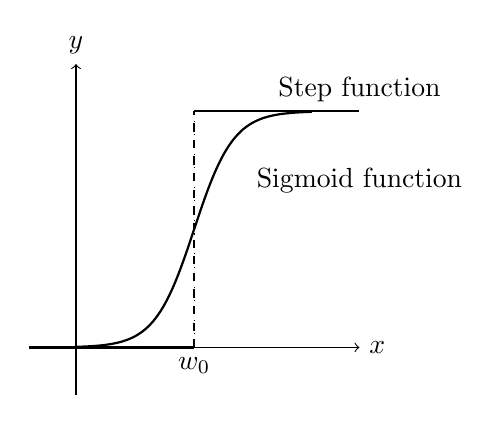
\begin{tikzpicture}[scale=3]
        % Axes
        \draw[->] (-0.2,0) -- (1.2,0) node[right] {$x$};
        \draw[->] (0,-0.2) -- (0,1.2) node[above] {$y$};

        % Step function (Perceptron)
        \draw[thick] (-0.2,0) -- (0.5,0);
        \draw[thick] (0.5,1) -- (1.2,1);
        \draw[thick,dashed] (0.5,0) -- (0.5,1);
        \node[above] at (1.2,1) {Step function};

        % Sigmoid function
        \draw[thick,domain=0:1,smooth,samples=100] plot
            (\x,{1/(1 + exp(-12*(\x - 0.5)))});
        \node[below] at (1.2,0.8) {Sigmoid function};

        % Threshold label
        \draw (0.5,0) node[below] {$w_0$};
        \draw[dotted] (0.5,0) -- (0.5,1);
    \end{tikzpicture}
    \caption{Perceptron and Sigmoid Neuron Output Characteristics.}
    \label{fig:step-sigmoid}
\end{figure}



\subsection{A Typical Supervised Machine Learning Setup}

We know that a typical supervised machine learning setup has the following components.

\begin{itemize}
    \item \textbf{Data:} A dataset of $n$ examples $\{(\mathbf{x}_i, y_i)\}_{i=1}^n$, where $\mathbf{x}_i$ are inputs and $y_i$ are corresponding outputs.
    \item \textbf{Model:} An approximation of the relation between input $\mathbf{x}$ and output $y$. For example,
    \[
    \hat{y} = \frac{1}{1 + e^{-\mathbf{w}^\top \mathbf{x}}}, \quad \hat{y} = \mathbf{w}^\top \mathbf{x}, \quad \hat{y} = \mathbf{x}^\top \mathbf{W} \mathbf{x}
    \]
    or any other function mapping inputs to outputs.
    \item \textbf{Parameters:} The model depends on parameters $\mathbf{w}$ (and possibly bias $b$) that need to be learned from the data.
    \item \textbf{Learning Algorithm:} A method to adjust parameters $\mathbf{w}$ and $b$ to fit the data. Examples include perceptron learning or gradient descent (we'll see gradient descent in detail in the next section).
    \item \textbf{Objective/Loss Function:} A function that measures the error of the model predictions. The learning algorithm aims to minimize this loss.
\end{itemize}

Consider data points $(x, y)$ where $x, y \in \mathbb{R}$. 
\[
\{(1,\ 0.05),\ (3,\ 0.15),\ (5,\ 0.4),\ (6,\ 0.6),\ (7,\ 0.65),\ (9,\ 0.85),\ (10,\ 0.95)\}
\]
Our model is 
\[
\hat{y} = \frac{1}{1 + e^{-(w x + b)}}
\]
We choose Mean Squared Error (MSE) as the loss function.
\[
\mathcal{L}(w, b) = \frac{1}{n} \sum_{i=1}^n \left( y_i - \hat{y}_i \right)^2
\]
This loss $\mathcal{L}(w,b)$ defines a surface over the two-dimensional parameter space $(w,b)$. Our goal is to find the $(w,b)$ that minimizes $\mathcal{L}$, the lowest point on this error surface.

Figure \ref{fig:3d_error_example} shows a 3D plot of the MSE loss surface as a function of $w$ and $b$ for the example data. 
 
\begin{figure}[h!]
    \centering
    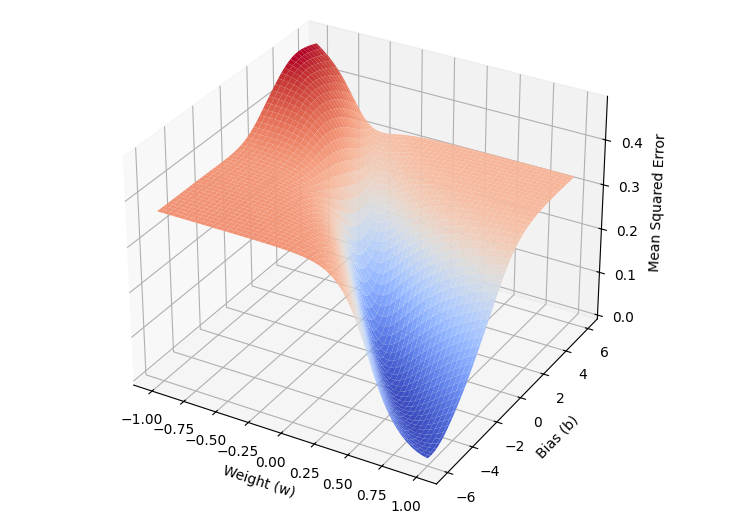
\includegraphics[width=0.7\textwidth]{content/section01/chapter01/figs/error_surface_sample.png}
    \caption{3D Error Surface Over Example Data}
    \label{fig:3d_error_example}
\end{figure}


\subsection{Sigmoid Neuron Learning Algorithm: Gradient Descent}

Let \( \boldsymbol{\theta} = [w, b] \) be the vector of parameters, initialized randomly. Suppose we move in the direction of a change \( \Delta \boldsymbol{\theta} = [\Delta w, \Delta b] \). Instead of making a full step, we scale the movement by a small scalar \( \eta \) to stay conservative. 
\[
\boldsymbol{\theta}_{\text{new}} = \boldsymbol{\theta} + \eta \cdot \Delta \boldsymbol{\theta}
\]

\textit{What is the right \( \Delta \boldsymbol{\theta} \) to choose?} \cite{khapra2018deeplearning}
To answer this, we turn to the Taylor series expansion. Let \( \boldsymbol{u} = \Delta \boldsymbol{\theta} \). Then the Taylor expansion of the loss function \( \mathcal{L}(\boldsymbol{\theta}) \) around \( \boldsymbol{\theta} \) is 
\[
\mathcal{L}(\boldsymbol{\theta} + \eta \boldsymbol{u}) = \mathcal{L}(\boldsymbol{\theta}) + \eta \cdot \boldsymbol{u}^T \nabla_{\boldsymbol{\theta}} \mathcal{L}(\boldsymbol{\theta}) + \frac{\eta^2}{2!} \cdot \boldsymbol{u}^T \nabla^2 \mathcal{L}(\boldsymbol{\theta}) \boldsymbol{u} + \frac{\eta^3}{3!} \cdot \ldots
\]
Since \( \eta \) is small, the higher-order terms are negligible.
\[
\mathcal{L}(\boldsymbol{\theta} + \eta \boldsymbol{u}) \approx \mathcal{L}(\boldsymbol{\theta}) + \eta \cdot \boldsymbol{u}^T \nabla_{\boldsymbol{\theta}} \mathcal{L}(\boldsymbol{\theta})
\]
For the move to reduce the loss, we require
\[
\mathcal{L}(\boldsymbol{\theta} + \eta \boldsymbol{u}) - \mathcal{L}(\boldsymbol{\theta}) < 0 \quad \Rightarrow \quad \boldsymbol{u}^T \nabla_{\boldsymbol{\theta}} \mathcal{L}(\boldsymbol{\theta}) < 0
\]
To understand how negative this term can be, consider the angle \( \beta \) between \( \boldsymbol{u} \) and \( \nabla_{\boldsymbol{\theta}} \mathcal{L}(\boldsymbol{\theta}) \). 
\[
\cos(\beta) = \frac{\boldsymbol{u}^T \nabla_{\boldsymbol{\theta}} \mathcal{L}(\boldsymbol{\theta})}{\|\boldsymbol{u}\| \cdot \| \nabla_{\boldsymbol{\theta}} \mathcal{L}(\boldsymbol{\theta}) \|} \text{ and } -1 \leq \cos(\beta) \leq 1
\]
Let \( k = \|\boldsymbol{u}\| \cdot \|\nabla_{\boldsymbol{\theta}} \mathcal{L}(\boldsymbol{\theta})\| \), then
\[
-k \leq \boldsymbol{u}^T \nabla_{\boldsymbol{\theta}} \mathcal{L}(\boldsymbol{\theta}) \leq k
\]
This implies that the most negative value is attained when \( \cos(\beta) = -1 \), i.e., when the angle is 180°.
\[
\boldsymbol{u} = -\nabla_{\boldsymbol{\theta}} \mathcal{L}(\boldsymbol{\theta})
\]

Hence, the \textit{gradient descent rule} says that the direction \( \boldsymbol{u} \) to move in should be opposite to the gradient of the loss.
\[
w_{t+1} = w_t - \eta \frac{\partial \mathcal{L}(w, b)}{\partial w}\bigg|_{w = w_t, b = b_t}
\quad \text{and} \quad
b_{t+1} = b_t - \eta \frac{\partial \mathcal{L}(w, b)}{\partial b}\bigg|_{w = w_t, b = b_t}
\]

\begin{algobox}{Gradient Descent Algorithm}
\( t \gets 0 \) \\
max iterations \( \gets 1000 \) \\
\textbf{while} \( t < \) max iterations \textbf{do} \\
\hspace*{1em} \( w_{t+1} \gets w_t - \eta \nabla_w \mathcal{L}(w_t, b_t) \) \\
\hspace*{1em} \( b_{t+1} \gets b_t - \eta \nabla_b \mathcal{L}(w_t, b_t) \) \\
\hspace*{1em} \( t \gets t + 1 \) \\
\textbf{end while}
\end{algobox}

Starting from initial values \( w = 0 \) and \( b = 0 \), gradient descent converges to final parameters \( w = 0.1487 \), \( b = -0.4139 \) with a final loss of \( 0.0527 \) after 100 iterations.\newpage

\begin{figure}[h!]
    \centering
    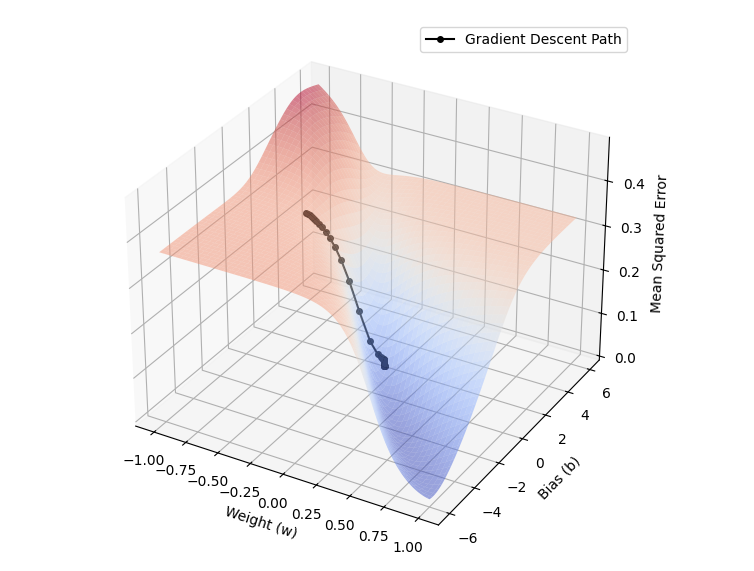
\includegraphics[width=0.7\textwidth]{content/section01/chapter01/figs/error_surface_grad_desc.png}
    \caption{Error Surface With Gradient Descent Trajectory.}
    \label{fig:gd_trajectory}
\end{figure}

\begin{figure}[h!]
    \centering
    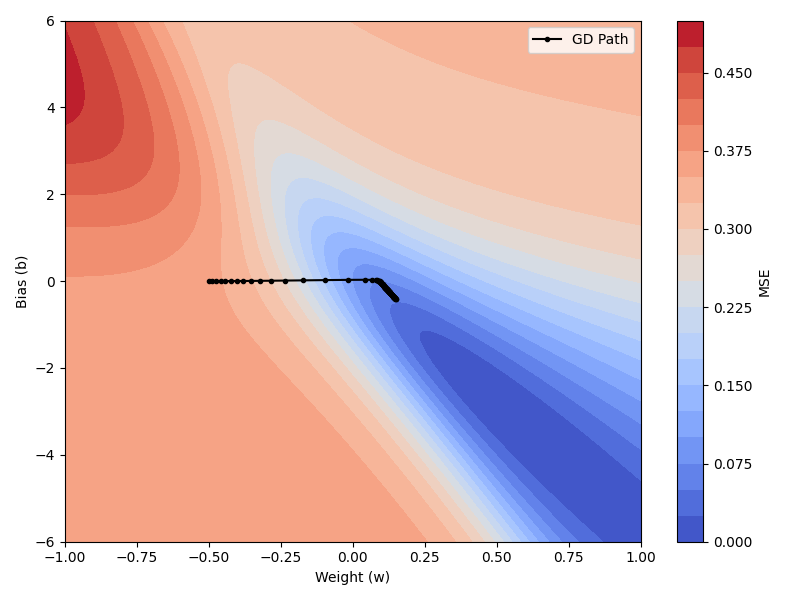
\includegraphics[width=0.65\textwidth]{content/section01/chapter01/figs/grad_desc_contour.png}
    \caption{Contour Plot of Gradient Descent Trajectory on Error Surface.}
\end{figure}

Visualizing in three dimensions can get cumbersome. So, we use 2D contour plots instead.  When the contours are close together, the slope is steep in that direction.  


\subsection{Momentum Based Gradient Descent}

Gradient descent can be slow in regions with gentle slopes. This happens because the gradient becomes very small, leading to small updates. To improve this, we can look at how updates behave over time.

The intuition is that if we keep getting asked to move in the same direction, it's reasonable to trust that direction and take bigger steps --- just like a ball gathers speed when rolling downhill.
\[
\text{update}_t = \gamma \cdot \text{update}_{t-1} + \eta \nabla w_t  
\]
\[
w_{t+1} = w_t - \text{update}_t
\]
Here, $\gamma$ is the momentum coefficient (typically between 0.5 and 0.9), and $\eta$ is the learning rate. This rule incorporates both the current gradient and the accumulated history of past gradients.
\begin{align*}
\text{update}_0 &= 0 \\
\text{update}_1 &= \gamma \cdot \text{update}_0 + \eta \nabla w_1 = \eta \nabla w_1 \\
\text{update}_2 &= \gamma \cdot \text{update}_1 + \eta \nabla w_2 = \gamma \cdot \eta \nabla w_1 + \eta \nabla w_2 \\
\text{update}_3 &= \gamma \cdot \text{update}_2 + \eta \nabla w_3 = \gamma^2 \cdot \eta \nabla w_1 + \gamma \cdot \eta \nabla w_2 + \eta \nabla w_3 \\
\text{update}_4 &= \gamma \cdot \text{update}_3 + \eta \nabla w_4 = \gamma^3 \cdot \eta \nabla w_1 + \gamma^2 \cdot \eta \nabla w_2 + \gamma \cdot \eta \nabla w_3 + \eta \nabla w_4
\end{align*}

Continuing this process, we can write the general form, 
\[
\text{update}_t = \sum_{k=1}^{t} \gamma^{\text{ }t-k} \cdot \eta \nabla w_k
\] 
This shows that updates are a weighted sum of all past gradients, with exponentially decaying weights controlled by $\gamma$.

\begin{algobox}{Momentum-based Gradient Descent Algorithm}
\( t \gets 0 \) \\
max iterations \( \gets 1000 \) \\
initialize updates: \( u^w_0 \gets 0, \quad u^b_0 \gets 0 \) \\
momentum coefficient \( \gamma \in [0,1) \) \\
learning rate \( \eta > 0 \) \\
\textbf{while} \( t < \) max iterations \textbf{do} \\
\hspace*{1em} \( u^w_{t+1} \gets \gamma \cdot u^w_t + \eta \nabla_w \mathcal{L}(w_t, b_t) \) \\
\hspace*{1em} \( u^b_{t+1} \gets \gamma \cdot u^b_t + \eta \nabla_b \mathcal{L}(w_t, b_t) \) \\
\hspace*{1em} \( w_{t+1} \gets w_t - u^w_{t+1} \) \\
\hspace*{1em} \( b_{t+1} \gets b_t - u^b_{t+1} \) \\
\hspace*{1em} \( t \gets t + 1 \) \\
\textbf{end while}
\end{algobox}


\begin{figure}[h!]
    \centering
    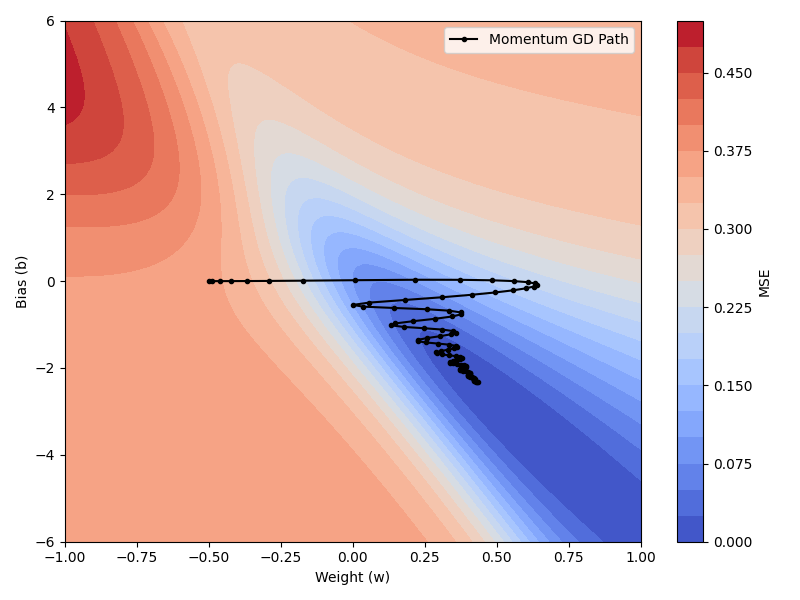
\includegraphics[width=0.65\textwidth]{content/section01/chapter01/figs/momentum_grad_desc_contour.png}
    \caption{Contour Plot of Momentum Gradient Descent Trajectory on Error Surface.}
\end{figure}

In our example, consider the initial values \( w = 0 \) and \( b = 0 \) and $\gamma = 0.9$. Momentum gradient descent converges to final parameters \( w = 0.4328 \), \( b = -2.3303 \) with a final loss of \( 0.004201 \) after 100 iterations. This surely performs better than the vanilla gradient descent. 

\subsection{Nesterov Accelerated Gradient Descent}

Even in regions with gentle slopes, momentum-based gradient descent takes large steps because momentum carries it forward. It oscillates in and out of the minima valley, often taking many U-turns before finally converging. Despite these oscillations, it converges faster than vanilla gradient descent. But \textit{can we reduce these oscillations?}

The intuition is to \textit{look before we leap}. Recall the momentum update equation,
\[
\text{update}_t = \gamma \cdot \text{update}_{t-1} + \eta \nabla_w \mathbf{w}_t
\]
We move at least by \(\gamma \cdot \text{update}_{t-1}\), plus a bit more by \(\eta \nabla_w \mathbf{w}_t\).

\textit{What if we calculate the gradient at a look-ahead point instead of the current position?} Let's say we define
\[
\mathbf{w}_{\text{look ahead}} = \mathbf{w}_t - \gamma \cdot \text{update}_{t-1}
\]
Then calculate the gradient \(\nabla_w \mathbf{w}_{\text{look ahead}}\) instead of \(\nabla_w \mathbf{w}_t\).

Thus, the update rule for Nesterov Accelerated Gradient (NAG) becomes
\[
\begin{aligned}
\mathbf{w}_{\text{look ahead}} &= \mathbf{w}_t - \gamma \cdot \text{update}_{t-1} \\
\text{update}_t &= \gamma \cdot \text{update}_{t-1} + \eta \nabla_w \mathbf{w}_{\text{look ahead}} \\
\mathbf{w}_{t+1} &= \mathbf{w}_t - \text{update}_t
\end{aligned}
\]

A similar update applies for the bias term \(b_t\).

\begin{algobox}{Nesterov Accelerated Gradient (NAG) Algorithm}
\( t \gets 0 \) \\
max iterations \( \gets 1000 \) \\
initialize \( \text{update}^w_{-1} \gets \mathbf{0} \), \( \text{update}^b_{-1} \gets 0 \) \\
momentum coefficient \( \gamma \in [0,1) \) \\
learning rate \( \eta > 0 \) \\

\textbf{while} \( t < \) max iterations \textbf{do} \\
\hspace*{1em} \(\mathbf{w}_{\text{look ahead}} \gets \mathbf{w}_t - \gamma \cdot \text{update}^w_{t-1}\) \\
\hspace*{1em} \(b_{\text{look ahead}} \gets b_t - \gamma \cdot \text{update}^b_{t-1}\) \\

\hspace*{1em} \(\text{update}^w_t \gets \gamma \cdot \text{update}^w_{t-1} + \eta \nabla_w \mathcal{L}(\mathbf{w}_{\text{look ahead}}, b_{\text{look ahead}})\) \\
\hspace*{1em} \(\text{update}^b_t \gets \gamma \cdot \text{update}^b_{t-1} + \eta \nabla_b \mathcal{L}(\mathbf{w}_{\text{look ahead}}, b_{\text{look ahead}})\) \\

\hspace*{1em} \(\mathbf{w}_{t+1} \gets \mathbf{w}_t - \text{update}^w_t\) \\
\hspace*{1em} \(b_{t+1} \gets b_t - \text{update}^b_t\) \\
\hspace*{1em} \( t \gets t + 1 \) \\
\textbf{end while}
\end{algobox}

\begin{figure}[h!]
    \centering
    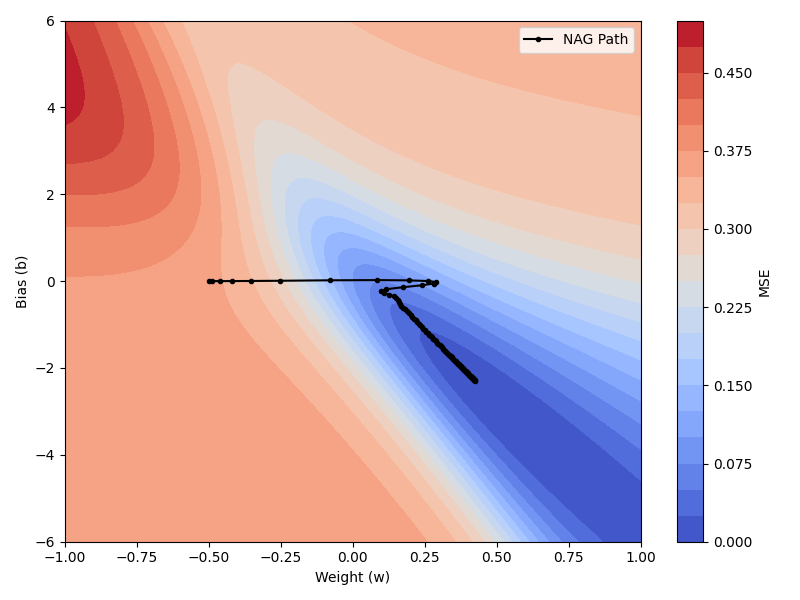
\includegraphics[width=0.65\textwidth]{content/section01/chapter01/figs/nesterov_grad_desc_contour.png}
    \caption{Contour Plot of Nesterov Gradient Descent Trajectory on Error Surface.}
\end{figure}

Looking ahead allows NAG to correct its course faster than momentum-based gradient descent. This reduces oscillations and lowers the chance of escaping the minima valley.

Starting from initial values \( w = 0 \) and \( b = 0 \), Nesterov Gradient Descent converges to final parameters \( w = 0.4247 \), \( b = -2.2946 \) with a final loss of \( 0.004477 \) after 100 iterations.

\subsection{Stochastic Gradient Descent}

Batch gradient descent computes the exact gradient of the loss by averaging the gradients over the entire dataset before updating the parameters. Because the full dataset is used, each update guarantees a decrease in the loss. 

However, this method becomes computationally expensive for large datasets. For example, with one million data points, one parameter update requires calculating one million gradients.

Stochastic Gradient Descent (SGD) improves efficiency by updating parameters after evaluating the gradient on each individual data point. Hence, for one million data points, SGD performs one million updates per epoch, where an \emph{epoch} is defined as a full pass over the dataset.

However, the gradient used in SGD is a noisy, stochastic estimate of the true gradient since it is computed using only one data point rather than the entire dataset. Due to this noise, there is no guarantee that each SGD update reduces the overall loss function. Indeed, the updates tend to oscillate, especially in small datasets, as each data point tries to optimize locally without considering the global effect on other points.

Even with these jumps, SGD can still find a good solution in the long run, as long as the learning rate is adjusted properly over time.

To smooth things out, we can use mini-batches. Instead of just one point, we use a small group of data points to compute the gradient. This reduces the noise while keeping the updates fast. It also helps the model converge more smoothly.

Also, the randomness in SGD isn’t always bad. It can help the model escape flat spots or shallow traps in the loss surface, which sometimes leads to better results.



\begin{algobox}{Mini-Batch Stochastic Gradient Descent Algorithm}
\( t \gets 0 \) \\
max iterations \( \gets 1000 \) \\
mini-batch size \( \gets m \) \\

\textbf{while} \( t < \) max iterations \textbf{do} \\
\hspace*{1em} Sample mini-batch \( \mathcal{B}_t \) of size \( m \) from training data \\

\hspace*{1em} Compute gradients over mini-batch: \\
\hspace*{2em} \( g_w \gets \frac{1}{m} \sum_{(x_i,y_i) \in \mathcal{B}_t} \nabla_w \mathcal{L}(w_t, b_t; \text{ }x_i, y_i) \) \\
\hspace*{2em} \( g_b \gets \frac{1}{m} \sum_{(x_i,y_i) \in \mathcal{B}_t} \nabla_b \mathcal{L}(w_t, b_t; \text{ }x_i, y_i) \) \\

\hspace*{2em} \( w_{t+1} \gets w_t - \eta g_w \) \\
\hspace*{2em} \( b_{t+1} \gets b_t - \eta g_b \) \\

\hspace*{1em} \( t \gets t + 1 \) \\
\textbf{end while}
\end{algobox}

Starting from initial values \( w = 0 \) and \( b = 0 \), Stochastic Gradient Descent converges to final parameters \( w = 0.3706 \), \( b = -1.9689 \) with a final loss of \( 0.007861 \) after 100 iterations.

\begin{figure}[h!]
    \centering
    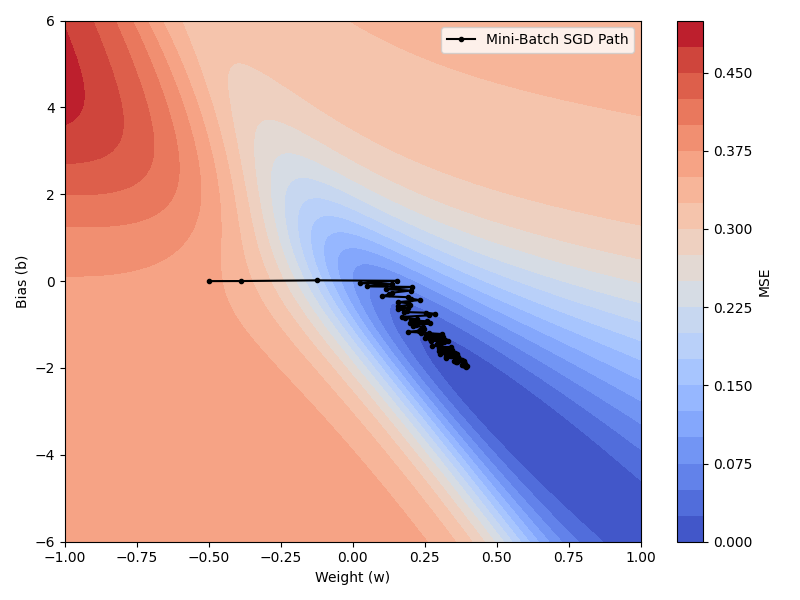
\includegraphics[width=0.65\textwidth]{content/section01/chapter01/figs/sgd_contour.png}
    \caption{Contour Plot of Stochastic Gradient Descent Trajectory on Error Surface.}
\end{figure}


\subsection{Gradient Descent with Adaptive Learning}

One might think to solve the problem of navigating gentle slopes by setting a high learning rate \( \eta \), effectively amplifying small gradients. But it is better to have a learning rate that adapts to the gradient itself.

\textbf{Intuition 1 (Adagrad):} Decay the learning rate for each parameter based on its past updates. More updates lead to more decay. The update rule for Adagrad is
\[
v_t = v_{t-1} + (\nabla w_t)^2
\]
\[
w_{t+1} = w_t - \frac{\eta}{\sqrt{v_t} + \epsilon} \cdot \nabla w_t
\]
A similar set of equations applies for the bias parameter \( b_t \).

\begin{algobox}{Batch Gradient Descent with Adagrad}
\( t \gets 0 \) , max iterations \( \gets 1000 \) \\
\( v_w \gets 0 \), \( v_b \gets 0 \) \\
\textbf{while} \( t < \) max iterations \textbf{do} \\
\hspace*{1em} \( g_{w_t} \gets \nabla_w \mathcal{L}(w_t, b_t) \) , \quad \( g_{b_t} \gets \nabla_b \mathcal{L}(w_t, b_t) \) \\
\hspace*{1em} \( v_w \gets v_w + g_{w_t}^2 \) , \quad \( v_b \gets v_b + g_{b_t}^2 \) \\
\hspace*{1em} \( w_{t+1} \gets w_t - \frac{\eta}{\sqrt{v_w} + \epsilon} \cdot g_{w_t} \) , \quad \( b_{t+1} \gets b_t - \frac{\eta}{\sqrt{v_b} + \epsilon} \cdot g_{b_t} \) \\
\hspace*{1em} \( t \gets t + 1 \) \\
\textbf{end while}
\end{algobox}


\begin{figure}[h!]
    \centering
    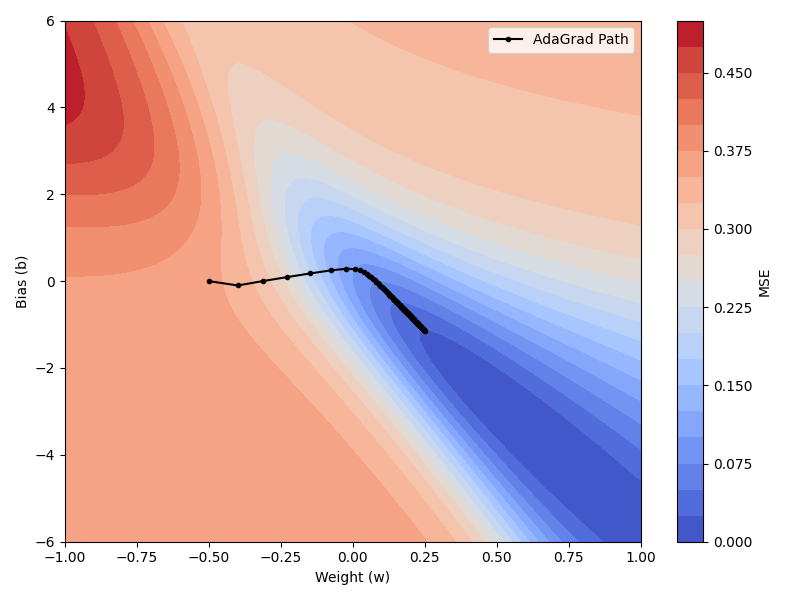
\includegraphics[width=0.65\textwidth]{content/section01/chapter01/figs/adagrad_gd_contour.png}
    \caption{Contour Plot of Gradient Descent Trajectory with Adagrad Learning on Error Surface.}
\end{figure}

Starting from initial values \( w = 0 \) and \( b = 0 \), Gradient Descent with Adagrad Learning converges to final parameters \( w = 0.2493 \), \( b = -1.1415 \) with a final loss of \( 0.024577 \) after 100 iterations.


\textbf{Intuition 2 (RMSProp):} Adagrad decays the learning rate too aggressively. After some time, frequently updated parameters get very small updates because the denominator \( \sqrt{v_t} \) grows without bound. To fix this, RMSProp decays \( v_t \) to prevent its rapid growth.

The update rule for RMSProp is
\[
v_t = \beta \cdot v_{t-1} + (1 - \beta) \cdot (\nabla w_t)^2
\]
\[
w_{t+1} = w_t - \frac{\eta}{\sqrt{v_t} + \epsilon} \cdot \nabla w_t
\]
Again, a similar set of equations applies for \( b_t \).

\begin{algobox}{Batch Gradient Descent with RMSProp}
\( t \gets 0 \) , max iterations \( \gets 1000 \) \\
Initialize \( v_w \gets 0 \), \( v_b \gets 0 \) \\
Choose \( \eta, \beta, \epsilon \) \\
\textbf{while} \( t < \) max iterations \textbf{do} \\
\hspace*{1em} \( g_w \gets \nabla_w \mathcal{L}(w_t, b_t) \),\quad \( g_b \gets \nabla_b \mathcal{L}(w_t, b_t) \) \\
\hspace*{1em} \( v_w \gets \beta \cdot v_w + (1 - \beta) \cdot g_w^2 \) , \quad \( v_b \gets \beta \cdot v_b + (1 - \beta) \cdot g_b^2 \) \\
\hspace*{1em} \( w_{t+1} \gets w_t - \frac{\eta}{\sqrt{v_w} + \epsilon} \cdot g_w \) , \quad \( b_{t+1} \gets b_t - \frac{\eta}{\sqrt{v_b} + \epsilon} \cdot g_b \) \\
\hspace*{1em} \( t \gets t + 1 \) \\
\textbf{end while}
\end{algobox}


Adagrad gets stuck near convergence because its learning rate decays too much, making it hard to move in some directions (like the vertical \( b \) direction). RMSProp fixes this by decaying \( v_t \) less aggressively.

\begin{figure}[h!]
    \centering
    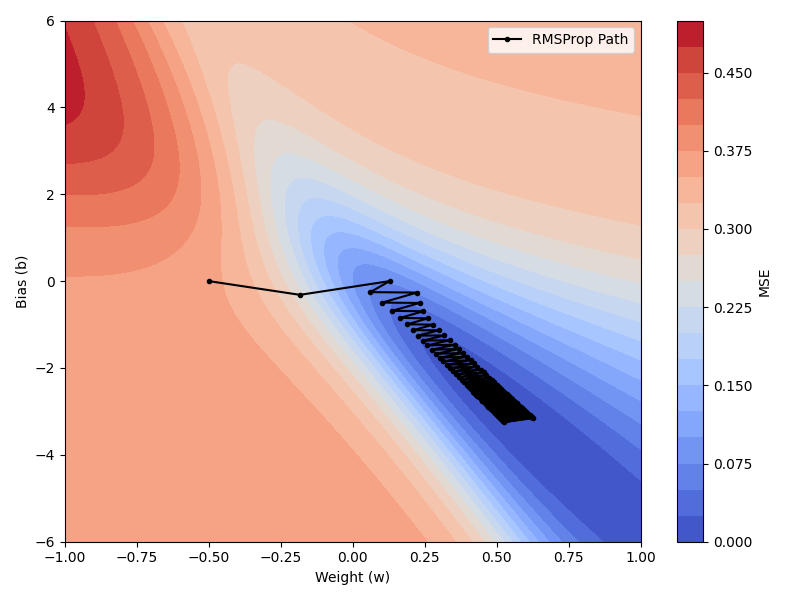
\includegraphics[width=0.7\textwidth]{content/section01/chapter01/figs/rmsprop_gd_contour.png}
    \caption{Contour Plot of Gradient Descent Trajectory with RMSProp Learning on Error Surface.}
\end{figure}

Starting from initial values \( w = 0 \) and \( b = 0 \), Gradient Descent with RMSProp Learning converges to final parameters \( w = 0.6249 \), \( b = -3.1551 \) with a final loss of \( 0.005095 \) after 100 iterations.

\textbf{Intuition 3 (Adam):} Adam builds on RMSProp by also keeping a cumulative history of gradients (first moment estimate).

The update rules for Adam are
\[
m_t = \beta_1 \cdot m_{t-1} + (1 - \beta_1) \cdot \nabla w_t
\]
\[
v_t = \beta_2 \cdot v_{t-1} + (1 - \beta_2) \cdot (\nabla w_t)^2
\]
\[
\hat{m}_t = \frac{m_t}{1 - \beta_1^t}
\]
\[
\hat{v}_t = \frac{v_t}{1 - \beta_2^t}
\]
\[
w_{t+1} = w_t - \frac{\eta}{\sqrt{\hat{v}_t} + \epsilon} \cdot \hat{m}_t
\]

A similar set of equations applies for \( b_t \).

Starting from initial values \( w = 0 \) and \( b = 0 \), Gradient Descent with Adam Learning converges to final parameters \( w = 0.5227 \), \( b = -2.9403 \) with a final loss of \( 0.001289 \) after 100 iterations.

\begin{algobox}{Batch Gradient Descent with Adam}
\( t \gets 0 \)  , \quad max iterations \( \gets 1000 \) \\
Initialize \( m_w = 0, \; v_w = 0, \; m_b = 0, \; v_b = 0 \) \\
Choose \(\beta_1, \beta_2\) \\

\textbf{while} \( t < \) max iterations \textbf{do} \\
\hspace*{1em} Compute gradients: \( g_w \gets \nabla_w \mathcal{L}(w_t, b_t) \), \( g_b \gets \nabla_b \mathcal{L}(w_t, b_t) \) \\

\hspace*{1em} \( m_w \gets \beta_1 \cdot m_w + (1 - \beta_1) \cdot g_w \) , \quad \( v_w \gets \beta_2 \cdot v_w + (1 - \beta_2) \cdot g_w^2 \) \\
\hspace*{1em} \( \hat{m}_w \gets \frac{m_w}{1 - \beta_1^t} \) , \quad \( \hat{v}_w \gets \frac{v_w}{1 - \beta_2^t} \) \\
\hspace*{1em} \( w_{t+1} \gets w_t - \frac{\eta}{\sqrt{\hat{v}_w} + \epsilon} \cdot \hat{m}_w \) \\

\hspace*{1em} \( m_b \gets \beta_1 \cdot m_b + (1 - \beta_1) \cdot g_b \) , \quad \( v_b \gets \beta_2 \cdot v_b + (1 - \beta_2) \cdot g_b^2 \) \\
\hspace*{1em} \( \hat{m}_b \gets \frac{m_b}{1 - \beta_1^t} \) , \quad \( \hat{v}_b \gets \frac{v_b}{1 - \beta_2^t} \) \\
\hspace*{1em} \( b_{t+1} \gets b_t - \frac{\eta}{\sqrt{\hat{v}_b} + \epsilon} \cdot \hat{m}_b \) \\

\hspace*{1em} \( t \gets t + 1 \) \\
\textbf{end while}
\end{algobox}


\begin{figure}[h!]
    \centering
    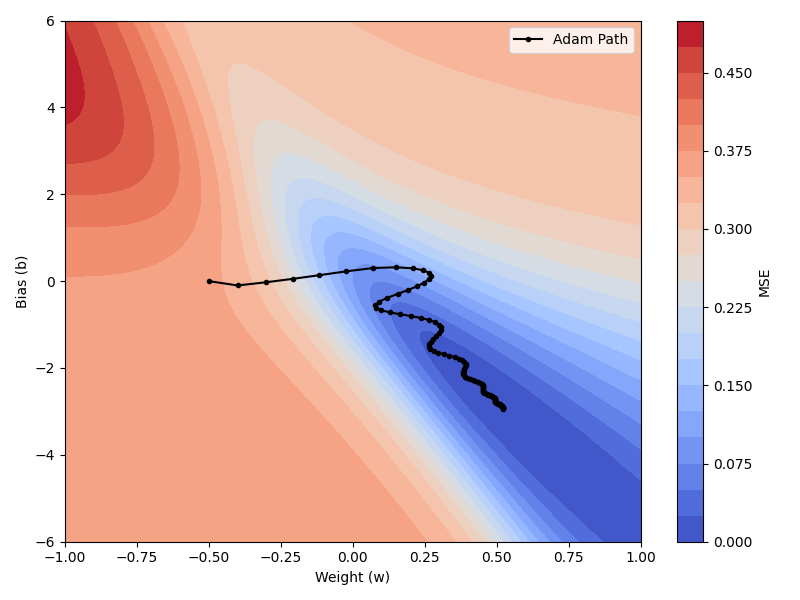
\includegraphics[width=0.7\textwidth]{content/section01/chapter01/figs/adam_gd_contour.png}
    \caption{Contour Plot of Gradient Descent Trajectory with Adam Learning on Error Surface.}
\end{figure}

All these adaptive learning rate methods modify the vanilla gradient descent update. Adam can also be combined with Nesterov's lookahead method for further improvements.

\begin{algobox}{Nesterov-Adam (Nadam) Algorithm}
\( t \gets 0 \), \quad max iterations \( \gets 1000 \) \\
Initialize \( m_w = 0, \; v_w = 0, \; m_b = 0, \; v_b = 0 \) \\
Initialize \( w_0, \; b_0 \), \quad momentum coefficient \( \gamma = \beta_1 \in [0,1) \), \quad learning rate \( \eta > 0 \) \\
\textbf{while} \( t < \) max iterations \textbf{do} \\
\hspace*{1em} \( \mathbf{w}_{\text{look ahead}} \gets \mathbf{w}_t - \gamma \cdot m_w \) \\
\hspace*{1em} \( b_{\text{look ahead}} \gets b_t - \gamma \cdot m_b \) \\
\hspace*{1em} Compute gradients: \( g_w \gets \nabla_w \mathcal{L}(\mathbf{w}_{\text{look ahead}}, b_{\text{look ahead}}) \), \quad \( g_b \gets \nabla_b \mathcal{L}(\mathbf{w}_{\text{look ahead}}, b_{\text{look ahead}}) \) \\

\hspace*{1em} \( m_w \gets \beta_1 \cdot m_w + (1 - \beta_1) \cdot g_w \) , \quad \( v_w \gets \beta_2 \cdot v_w + (1 - \beta_2) \cdot g_w^2 \) \\
\hspace*{1em} \( \hat{m}_w \gets \frac{m_w}{1 - \beta_1^{t+1}} \) , \quad \( \hat{v}_w \gets \frac{v_w}{1 - \beta_2^{t+1}} \) \\
\hspace*{1em} \( w_{t+1} \gets w_t - \frac{\eta}{\sqrt{\hat{v}_w} + \epsilon} \cdot (\gamma \cdot \hat{m}_w + (1 - \gamma) \cdot g_w) \) \\

\hspace*{1em} \( m_b \gets \beta_1 \cdot m_b + (1 - \beta_1) \cdot g_b \) , \quad \( v_b \gets \beta_2 \cdot v_b + (1 - \beta_2) \cdot g_b^2 \) \\
\hspace*{1em} \( \hat{m}_b \gets \frac{m_b}{1 - \beta_1^{t+1}} \) , \quad \( \hat{v}_b \gets \frac{v_b}{1 - \beta_2^{t+1}} \) \\
\hspace*{1em} \( b_{t+1} \gets b_t - \frac{\eta}{\sqrt{\hat{v}_b} + \epsilon} \cdot (\gamma \cdot \hat{m}_b + (1 - \gamma) \cdot g_b) \) \\
\hspace*{1em} \( t \gets t + 1 \) \\
\textbf{end while}
\end{algobox}


\begin{figure}[h!]
    \centering
    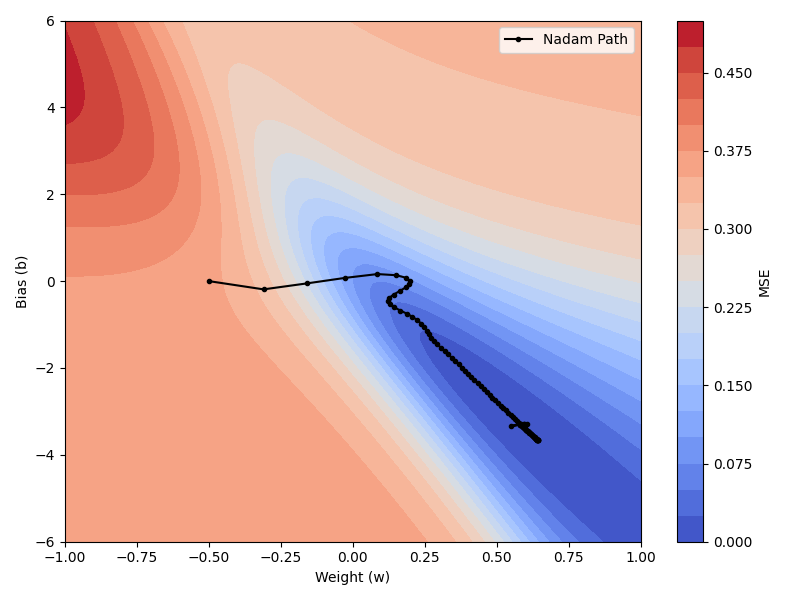
\includegraphics[width=0.7\textwidth]{content/section01/chapter01/figs/nadam.png}
    \caption{Contour Plot of Nesterov Gradient Descent Trajectory with Adam Learning on Error Surface.}
\end{figure}

Starting from initial values \( w = 0 \) and \( b = 0 \), Nesterov Gradient Descent with Adam Learning converges to final parameters \( w = 0.5829 \), \( b = -3.3043 \) with a final loss of \( 0.000833 \) after 100 iterations.

\begin{table}[h!]
\centering
\begin{tabular}{|l|c|c|c|}
\hline
\textbf{Method} & \textbf{Final Parameters (w, b)} & \textbf{Final Loss} \\ \hline
Vanilla Gradient Descent & \( w = 0.1487,\; b = -0.4139 \) & 0.0527 \\ \hline
Momentum Gradient Descent (\( \gamma = 0.9 \)) & \( w = 0.4328,\; b = -2.3303 \) & 0.004201 \\ \hline
Nesterov Gradient Descent & \( w = 0.4247,\; b = -2.2946 \) & 0.004477 \\ \hline
Stochastic Gradient Descent & \( w = 0.3706,\; b = -1.9689 \) & 0.007861 \\ \hline
Adagrad Gradient Descent & \( w = 0.2493,\; b = -1.1415 \) & 0.024577 \\ \hline
RMSProp Gradient Descent & \( w = 0.6249,\; b = -3.1551 \) & 0.005095 \\ \hline
Adam Gradient Descent & \( w = 0.5227,\; b = -2.9403 \) & 0.001289 \\ \hline
\textbf{Nesterov with Adam (Best)} & \textbf{\( w = 0.5829,\; b = -3.3043 \)} & \textbf{0.000833} \\ \hline
\end{tabular}
\caption{Comparison of Gradient Descent Methods (Initial values: \( w = 0 \), \( b = 0 \), 100 iterations)}
\end{table}


\subsection{Layer of Sigmoid Neurons}

Recall a multilayer network of perceptrons with a single hidden layer can be used to represent any boolean function precisely (no errors). Similarly, the representation power of a multilayer network of sigmoid neurons is given by the \textbf{Universal Approximation Theorem.} To prove this, we will need the result from \textbf{Stone-Weierstrass Theorem}. 

\begin{theorem}
    \label{thm:stone-weierstrass}
    \textbf{Stone-Weierstrass Theorem}. Let $K$ be a compact subset of $\mathbb{R}^n$ and let $\mathcal{A}$ be a subalgebra of $C(K)$ (the space of continuous real-valued functions on $K$) such that 
\begin{enumerate}
    \item $\mathcal{A}$ separates points of $K$ (i.e., for any $x, y \in K$ with $x \neq y$, there exists $f \in \mathcal{A}$ such that $f(x) \neq f(y)$)
    \item $\mathcal{A}$ contains the constant functions
\end{enumerate}
Then $\mathcal{A}$ is dense in $C(K)$ with respect to the uniform norm.
\end{theorem}

Imagine you have a collection of continuous functions defined on a \textit{nice} and \textit{closed} space (like a closed and bounded interval). If this collection of functions has two key properties:
\begin{enumerate}
    \item \textit{They can tell points apart}. For any two distinct points in your space, you can find a function in your collection that gives different values for those two points.
    \item \textit{They include all the constant functions}. You have functions in your collection that are just a fixed number everywhere.
\end{enumerate}
Then, you can use combinations of these functions (adding them, multiplying them, multiplying them by constants) to get arbitrarily close to any other continuous function on that space.

Essentially, if your initial collection of functions is rich enough to distinguish between points and includes constants, it's \textit{dense} enough to build approximations for any other continuous function you can think of on that space.

\begin{proof}
Let \( f \in C(K) \) and \( \varepsilon > 0 \). We aim to show that there exists a function \( g \in \mathcal{A} \) such that 
\[
\|f - g\|_\infty < \varepsilon.
\]

\textbf{Step 1: Approximate indicator functions.}

Fix \( x_0 \in K \). For any \( x \in K \), since \( \mathcal{A} \) separates points, there exists \( \phi_x \in \mathcal{A} \) such that \( \phi_x(x) \neq \phi_x(x_0) \). Define:
\[
\psi_x(y) = \left( \frac{\phi_x(y) - \phi_x(x_0)}{\phi_x(x) - \phi_x(x_0)} \right)^2.
\]
Then \( \psi_x \in \mathcal{A} \) because \( \mathcal{A} \) is a subalgebra (closed under addition, multiplication, and scalar multiplication), and we’ve used only these operations. Also, \( \psi_x(x_0) = 0 \), and \( \psi_x(x) = 1 \).

Now, for a finite set \( \{x_1, \dots, x_m\} \subset K \), we can construct a partition of unity-like approximation by defining functions \( \{\psi_{x_j}\}_{j=1}^m \) and then normalize
\[
S(y) = \sum_{j=1}^m \psi_{x_j}(y), \quad \rho_j(y) = \frac{\psi_{x_j}(y)}{S(y)}.
\]
Each \( \rho_j \in \mathcal{A} \), and \( \sum_{j=1}^m \rho_j(y) = 1 \) for all \( y \in K \).

\textbf{Step 2: Local approximation of \( f \).}

Since \( f \) is uniformly continuous on compact \( K \), there exists a finite \( \delta \)-net \( \{x_1, \dots, x_m\} \subset K \) such that for all \( y \in K \), there exists \( x_j \) with \( |f(y) - f(x_j)| < \varepsilon \). 

Now define the function
\[
g(y) = \sum_{j=1}^m f(x_j) \rho_j(y).
\]
Then \( g \in \mathcal{A} \) because \( \rho_j \in \mathcal{A} \) and \( f(x_j) \) are constants (constants are in \( \mathcal{A} \), and the algebra is closed under scalar multiplication and addition).

\textbf{Step 3: Approximation bound.}

We estimate the uniform difference
\[
|f(y) - g(y)| = \left|f(y) - \sum_{j=1}^m f(x_j) \rho_j(y)\right| = \left|\sum_{j=1}^m \rho_j(y) (f(y) - f(x_j))\right|.
\]
Using the triangle inequality
\[
|f(y) - g(y)| \leq \sum_{j=1}^m \rho_j(y) |f(y) - f(x_j)|.
\]
Since each \( \rho_j(y) \geq 0 \), and \( \sum \rho_j(y) = 1 \), this is a convex combination of errors \( |f(y) - f(x_j)| \), each less than \( \varepsilon \). So,
\[
|f(y) - g(y)| < \varepsilon \quad \text{for all } y \in K.
\]
Hence,
\[
\|f - g\|_\infty < \varepsilon.
\]
\end{proof}

\begin{example}
    Polynomials can be used to approximate any continuous function on a closed interval.
\end{example}

\begin{solution}
Let $K$ be a compact subset of $\mathbb{R}^n$. We consider the subalgebra $\mathcal{A}$ of $C(K)$ consisting of all polynomial functions on $K$. For clarity, let's first consider the common case where $K$ is a closed and bounded interval in $\mathbb{R}$, say $K = [a, b]$.

A function $f \in \mathcal{A}$ has the form $f(x) = c_m x^m + c_{m-1} x^{m-1} + \dots + c_1 x + c_0$ for some non-negative integer $m$ and real coefficients $c_0, c_1, \dots, c_m$.

We need to demonstrate that $\mathcal{A}$ satisfies the two properties required by the Stone-Weierstrass Theorem.

\textbf{1. $\mathcal{A}$ separates points of $K$}

This property requires that for any distinct points $x, y \in K$ (i.e., $x \neq y$), there must exist a function $f \in \mathcal{A}$ such that $f(x) \neq f(y)$.

Consider any two distinct points $x, y \in [a, b]$ such that $x \neq y$.
Let's choose the polynomial function $f(t) = t$. This is a simple polynomial of degree 1 (where $m=1$, $c_1=1$, and $c_0=0$).
Evaluating this function at $x$ and $y$, we get $f(x) = x$ and $f(y) = y$.
Since we initially assumed $x \neq y$, it directly follows that $f(x) \neq f(y)$.

Therefore, the set of polynomial functions $\mathcal{A}$ successfully separates points of $K$.

\textbf{2. $\mathcal{A}$ contains the constant functions}

This property requires that for any real number $c$, the constant function $g(t) = c$ for all $t \in K$ must be an element of $\mathcal{A}$.

A constant function $g(t) = c$ can be expressed as a polynomial of degree 0. We can write $g(t) = c \cdot t^0$, or simply $g(t) = c$. This fits the general form of a polynomial where $m=0$ and $c_0=c$.

Thus, for any real number $c$, the constant function $g(t)=c$ is indeed a polynomial.

Therefore, the set of polynomial functions $\mathcal{A}$ contains all constant functions.

Since the set of polynomial functions on $K=[a,b]$ satisfies both of these crucial properties, the Stone-Weierstrass Theorem implies that the set of polynomials is \textbf{dense} in $C([a,b])$. 
\end{solution}

This is a fundamental result, meaning that any continuous real-valued function defined on a closed and bounded interval can be uniformly approximated arbitrarily well by polynomials. The argument extends naturally to compact subsets of $\mathbb{R}^n$. In this case, $\mathcal{A}$ would comprise polynomials in $n$ variables.


Refer figure \ref{fig:stone-weierstrass} for illustration.

\begin{figure}[h]
\centering
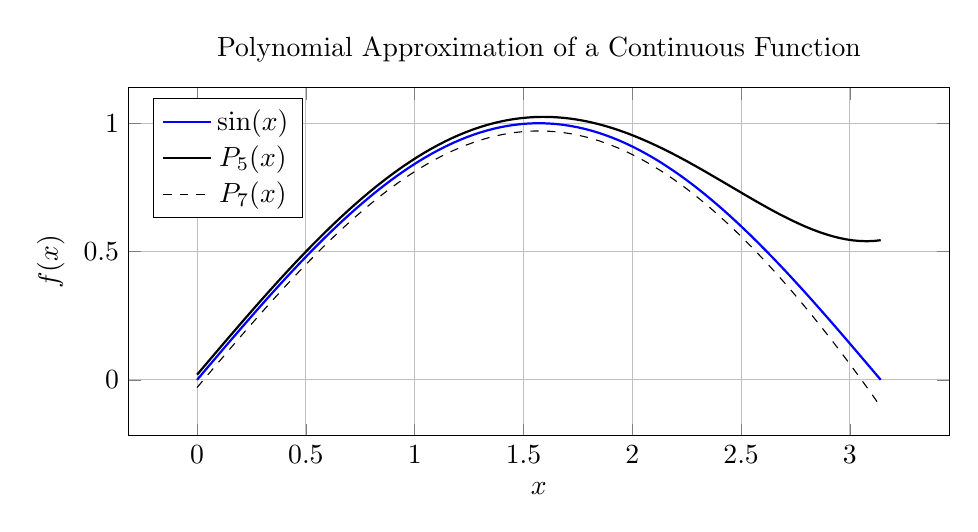
\begin{tikzpicture}
\begin{axis}[
    width=12cm,
    height=6cm,
    xlabel={$x$},
    ylabel={$f(x)$},
    title={Polynomial Approximation of a Continuous Function},
    grid=major,
    legend pos=north west,
    domain=0:pi,
    samples=100
]
\addplot[blue, thick] {sin(deg(x))};
\addplot[black, thick] {x - x^3/6 + x^5/120 + 0.02};
\addplot[black, dashed] {x - x^3/6 + x^5/120 - x^7/5040 - 0.03};
\legend{$\sin(x)$, $P_5(x)$, $P_7(x)$}
\end{axis}
\end{tikzpicture}
\caption{Illustration of the Stone-Weierstrass theorem. Polynomials $P_5(x)$ and $P_7(x)$ successively approximate $\sin(x)$ with increasing accuracy on the compact interval $[0, \pi]$.}
\label{fig:stone-weierstrass}
\end{figure}

\begin{theorem}
    \textbf{Universal Approximation Theorem.} Let $\sigma: \mathbb{R} \to \mathbb{R}$ be a non-constant, bounded, and continuous function (such as the sigmoid function). Let $K \subset \mathbb{R}^n$ be compact. Then for any continuous function $f: K \to \mathbb{R}$ and any $\varepsilon > 0$, there exist $N \in \mathbb{N}$, weights $\alpha_1, \ldots, \alpha_N \in \mathbb{R}$, weight vectors $\mathbf{w}_1, \ldots, \mathbf{w}_N \in \mathbb{R}^n$, and biases $b_1, \ldots, b_N \in \mathbb{R}$ such that the function
\[
g(\mathbf{x}) = \sum_{j=1}^{N} \alpha_j \sigma(\mathbf{w}_j^T \mathbf{x} + b_j)
\]
satisfies $\sup_{\mathbf{x} \in K} |f(\mathbf{x}) - g(\mathbf{x})| < \varepsilon$.
\end{theorem}

\begin{proof}
We want to show that the set of functions
\[
\mathcal{F} = \left\{ \sum_{j=1}^{N} \alpha_j \sigma(\mathbf{w}_j^T \mathbf{x} + b_j) : N \in \mathbb{N}, \text{ } \alpha_j \in \mathbb{R}, \text{ }\mathbf{w}_j \in \mathbb{R}^n, \text{ }b_j \in \mathbb{R} \right\}
\]
is dense in \( C(K) \), the space of continuous real-valued functions on compact \( K \subset \mathbb{R}^n \), with respect to the uniform norm.
Let us define
\[
\mathcal{A} = \text{span}\{ \sigma(\mathbf{w}^T \mathbf{x} + b) : \mathbf{w} \in \mathbb{R}^n, b \in \mathbb{R} \},
\]
which is a subalgebra of \( C(K) \). 

\textbf{Step 1: Closure under addition, multiplication, and scalar multiplication.}

The set \( \mathcal{A} \) is a linear span of compositions of affine functions with \( \sigma \), so it is closed under addition and scalar multiplication by construction. 

\textbf{Step 2: Separation of points.}

Let \( \mathbf{x}, \mathbf{y} \in K \) with \( \mathbf{x} \neq \mathbf{y} \). Since \( \sigma \) is non-constant and continuous, there exists a hyperplane (i.e., choice of \( \mathbf{w} \in \mathbb{R}^n \)) such that \( \mathbf{w}^T \mathbf{x} \neq \mathbf{w}^T \mathbf{y} \). Then for any fixed \( b \), we have
\[
\sigma(\mathbf{w}^T \mathbf{x} + b) \neq \sigma(\mathbf{w}^T \mathbf{y} + b),
\]
because \( \sigma \) is strictly increasing (as in sigmoid), or at least non-constant and continuous, so it distinguishes between different inputs. Hence, \( \mathcal{A} \) separates points of \( K \).

\textbf{Step 3: Constants are in \( \mathcal{A} \).}

Since \( \sigma \) is bounded and non-constant, it attains at least two values. For large positive or negative arguments, \( \sigma(z) \to c_1 \) or \( c_2 \), so we can scale and shift \( \sigma \) to approximate constant functions arbitrarily well. More directly, linear combinations of shifted sigmoids can approximate any constant function.
Hence, \( \mathcal{A} \) contains constant functions or can approximate them arbitrarily well, which is enough for density in the uniform norm.

By the Stone-Weierstrass Theorem~\ref{thm:stone-weierstrass}, \( \mathcal{A} \) is dense in \( C(K) \). Thus, for any \( f \in C(K) \) and \( \varepsilon > 0 \), there exists a finite sum of the form
\[
g(\mathbf{x}) = \sum_{j=1}^{N} \alpha_j \sigma(\mathbf{w}_j^T \mathbf{x} + b_j)
\]
such that
\[
\sup_{\mathbf{x} \in K} |f(\mathbf{x}) - g(\mathbf{x})| < \varepsilon.
\]
\end{proof}


\begin{corollary}
    A multilayer network of neurons with a single hidden layer can be used to approximate any continuous function to any desired precision. 
\end{corollary}

In other words, there is a guarantee that for any function \( f(\mathbf{x}) : \mathbb{R}^n \to \mathbb{R}^m \), we can always find a neural network (with one hidden layer containing enough sigmoid neurons) whose output \( g(\mathbf{x}) \) satisfies \( |g(\mathbf{x}) - f(\mathbf{x})| < \varepsilon \).
